\documentclass[11pt]{article}
\usepackage[utf8]{inputenc}
\usepackage[pdftex]{graphicx}
\usepackage{pdfpages}
\usepackage[english]{babel}
\usepackage [autostyle, english = american]{csquotes}
\usepackage{mathtools}
\usepackage{float}
\usepackage{xcolor}
\usepackage{listings}
\usepackage{fancyvrb}
\usepackage{caption,subcaption}
%\usepackage{subfigure}
\usepackage[margin=0.6in]{geometry}
\usepackage{adjustbox}
\usepackage{listings}
\usepackage{hyperref}
\usepackage{wrapfig}
\usepackage{newfloat}
\usepackage[cm]{fullpage}
\usepackage[cachedir=build,newfloat,outputdir=build]{minted}
\usepackage{verbatim}

\definecolor{mintedbackground}{rgb}{0,0,0}
\usemintedstyle{tango}
\newenvironment{code}{\captionsetup{type=listing}}{}
\SetupFloatingEnvironment{listing}{name=Source Code}
\captionsetup[subfigure]{subrefformat=simple,labelformat=simple}
\renewcommand{\thelisting}{\arabic{listing}}
\renewcommand\thesubfigure{(\alph{subfigure})}
\definecolor{lightgray}{rgb}{.7,.7,.7}
\definecolor{gray}{rgb}{.4,.4,.4}
\definecolor{darkblue}{rgb}{0,0,.3}
\definecolor{gray}{rgb}{0.4,0.4,0.4}
\definecolor{darkblue}{rgb}{0.0,0.0,0.6}
\definecolor{cyan}{rgb}{0.0,0.6,0.6}
\renewcommand{\thelisting}{\arabic{listing}}
\renewcommand\thesubfigure{(\alph{subfigure})}

\definecolor{termback}{HTML}{DBE0E0}
\definecolor{termkeyword}{HTML}{50DA8B}
\lstdefinestyle{Bash}
{language=bash,
keywordstyle=\color{termkeyword},
basicstyle=\ttfamily,
morekeywords={@.},
alsoletter={:~\$.},
morekeywords=[2]{peter@kbpet:},
keywordstyle=[2]{\color{termkeyword}},
literate={\$}{{\textcolor{termkeyword}{\$}}}1 
         {:}{{\textcolor{termkeyword}{:}}}1
         {~}{{\textcolor{termkeyword}{\textasciitilde}}}1,
}

\geometry{
 a4paper,
 total={170mm,257mm},
 left=10mm,
 right=10mm,
 top=10mm,
 bottom=15mm
}
\graphicspath{ {code/} }

\lstset{
  basicstyle=\ttfamily,
  columns=fullflexible,
  showstringspaces=false,
  commentstyle=\color{gray}\upshape
}

\hypersetup{
    colorlinks,
    citecolor=black,
    filecolor=black,
    linkcolor=black,
    urlcolor=blue
}
 \newmintedfile[pycode]{python3}{
frame=lines,
framesep=2mm,
fontsize=\footnotesize,
showtabs =false,
autogobble=true,
breaklines=true,
mathescape=true
}
 \newmintedfile[shellcode]{bash}{
frame=lines,
framesep=2mm,
fontsize=\footnotesize,
showtabs =false,
autogobble=true,
breaklines=true,
mathescape=true
}


\newmintinline[ibash]{bash} {
}
\RecustomVerbatimCommand{\VerbatimInput}{VerbatimInput}%
{fontsize=\footnotesize,
 %
 frame=lines,  % top and bottom rule only
 framesep=2em, % separation between frame and text
 %
 labelposition=topline,
 %
 commandchars=\|\(\), % escape character and argument delimiters for
                      % commands within the verbatim
 commentchar=*        % comment character
}

\title{Assignment 3 \\ Introduction to Information Retrieval \\ CS734/834}
\author{John Berlin}
\date{\today}
\renewcommand\thesection{Q.\arabic{section}}
\renewcommand\thesubsection{\thesection}
\begin{document}
\maketitle
\newpage
\section*{Note}
As was mentioned in the this section for assignment two the size considerations for output files apply generated for this assignment.
The trec files produces by \textit{batch-search} and the indexes created by \textit{build} functions of galago prohibit them from inclusion in this report. Also used in this report the shell script \textit{rungalago.sh}, \autoref{code:rg}, was used to streamline the usage of galago by providing the argument boiler plate to command which required more than path arguments and to run the bin script for galago which resides in the nested directory structure of the application.  The two commands which required the argument boiler plate are build and build-window both create a search index whereas the latter creates a windowed version of the first. \newline 
The version of galago used in this report is 3.10, which was rebuilt from source, whereas the version available via the link found on the textbooks \href{http://www.search-engines-book.com/}{web-site} is version 1.04 built in 2009. Even tho galago is a Java application, it was found that this version suffered from performance issues due to its age. The biggest difference in 3.10 from 1.04 is that batch queries are in JSON format not XML and all other changes are minor feature additions and performance increases.
\newpage
\section{Question 4.2} \label{q1}
\begin{verbatim}
6.1. Using the Wikipedia collection provided at the book website, create a sample
of stem clusters by the following process:
1. Index the collection without stemming.
2. Identify the first 1,000 words (in alphabetical order) in the index.
3. Create stem classes by stemming these 1,000 words and recording which
words become the same stem.
4. Compute association measures (Dice’s coefficient) between all pairs of stems
in each stem class. Compute co-occurrence at the document level.
5. Create stem clusters by thresholding the association measure. All terms that
are still connected to each other form the clusters.
Compare the stem clusters to the stem classes in terms of size and the quality (in
your opinion) of the groupings.
\end{verbatim}
\subsection{Answer} 
The first step was to create the index for the Wikipedia collection by executing the command \newline \ibash{./rungalago.sh build index htmls} where the first argument index is the location to where the index is to be placed and htmls is the location of the input. The html files of the Wikipedia collection were moved to a single directory as galago took some time to traverse the original directory structure of this data set which contained 6,042 files. As was mentioned in the note section the build command required argument boilerplate and was executed with the following addition arguments supplied by the script: \newline \ibash{--nonStemmedPosting=true --stemmedPostings=true --stemmer+krovetz --corpus=true}. By passing the arguments nonStemmedPostings and stemmedPostings galago created separate index files for both index types. Indexing the collection was surprisingly quick as shown in the report generated once indexing has finished \autoref{fig:q1idxreport}. After the build was complete the python file indexer.py, \autoref{code:idxr}, was used to dump the index file and extract terms.
\begin{figure}[H]
\centering
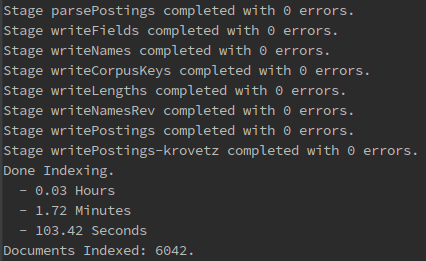
\includegraphics[scale=0.8]{indexingReport.png}
\caption{Indexing Report}
\label{fig:q1idxreport}
\end{figure}
\begin{figure}[H]
\centering
\includegraphics[scale=0.5]{q1Run.png}
\caption{Python Output}
\label{fig:q1Run}
\end{figure}
\noindent After the index was built the python file q1\_6dot1run.py, \autoref{code:scd}, was used to generate the results for this question. Running the file produced the output seen in \autoref{fig:q1Run}. This python script expects the directories \textit{output\_files} and \textit{pickled} to be present in the working directory the script is executed at using \ibash{python3 q1_6dot1run.py}. The first 1000 words in the collection only began with the letter \textit{a} which I found to lead to un-interesting results. To augment this I stemmed the entire index using four different stemmers: Porter, Snowball, WordnetLemmatizer, and Lancaster which are available via the nltk.stem package. This was achieved by using the pseq (parallel sequence)  function from the pyfunctional package which made the processing timely. Processing the data used the \textit{flatmap} function in parallel to transform the was utilized to transform the list of tuples (StemmerName,Stem,Word) to single list then foldleft was used to accumulate the tuples into Stemmer[Stem][words] structure. After which the stem classes for a stemmer were written to files with name idx\_[Stemmer].txt .  \newline \newline \noindent
Computing Dice's coefficient and co-occurrence at document level was done by constructing queries run via galago threaded-batch-search. After the queries were written and serialized to disk after which they were executed via the python code for this question and the trec file format returned by galago were also written to disk. A total of 1,453,423 queries were created of which Lancaster had 694,985, WordNetLemmatizer had 184,843, Porter had 286,350, and  Snowball had 287,245. Calculation for Dice's coefficient required a slight modification due to the combine operator being an \href{https://sourceforge.net/p/lemur/wiki/Belief Operations/}{or operation} which was to subtract the counts for a and b from the addition of the individual counts for the word pairs. The filter threshold was set at $0.001$ due to the relatively small number of documents in this collection and each stemmers results were written to files with name Stemmer\_dice.txt and Stemmer\_dice\_filtered.txt. The final step was to generate the report for the new stem classes \autoref{q1:report}.
\newline \newline \noindent To my surprise each stem class created each one contained the same number of words as the original stemming contained. The scores seen in \autoref{q1:report} are from the cumulative scores for all stems classes which was calculated by taking the sum of the each word pairs Dice score and dividing it by the number of pairs contained in the new stem class if the stem class had more than one pair. Also of note the stems not in the new stem classes the number of words for each was one to two.
\lstinputlisting[caption=Stem Class Dice Filtered Report, label=q1:report]{code/q1report.txt}
Now to ensure this was not off I looked for the stem \textit{admir} in all the generated classes. All but WordNetLemmatizer contained this stem as seen in \autoref{q1:rsame}.
\lstinputlisting[breaklines=true,caption=Stem Class Dice Filtered Report, label=q1:rsame]{code/same.txt}
But when grepping for that stem, \autoref{fig:grep}, it is clear to see WordNet does not do what one might think if not looking into the kind of stemming it does. For instance \textit{/do do dos} the lemmatization works well. But for \textit{/doje doje} and \textit{/dojo dojo} it does not as both would be expected to stem to \textit{doj} at least. But lemmatisation \footnote{https://en.wikipedia.org/wiki/Lemmatisation} is the process of grouping together the inflected forms of a word so they can be analysed as a single item, identified by the word's lemma, or dictionary form  
\begin{figure}[H]
\centering
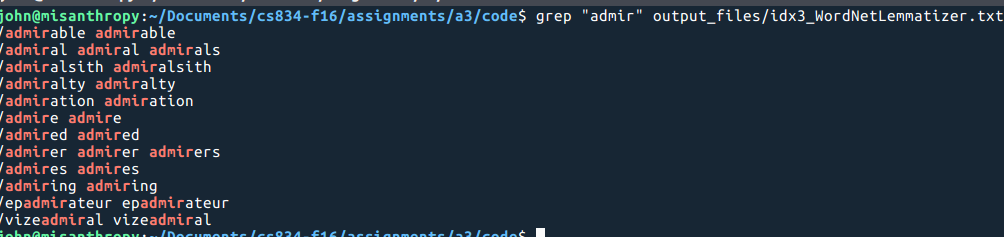
\includegraphics[scale=0.5]{grepOutput.png}
\caption{Grep WordNet admir}
\label{fig:grep}
\end{figure}
\newpage
\begin{code}
\captionof{listing}{Extract Terms From Index} \label{code:idxr}
	\pycode{code/indexer.py}
\end{code}
\begin{code}
\captionof{listing}{Stem Cluser Generation Dice} \label{code:scd}
	\pycode{code/q1_6dot1.py}
\end{code}
\newpage
\section{MLN1}
\begin{verbatim}
using the small wikipedia example, choose 10 words 
and create stem classes as per the algorithm on pp. 191-192
\end{verbatim}
\subsection{Answer}
This question builds heavily on the work done in question one and uses the work done by \autoref{q1} up to the generation of the stem classes which is where I will focus on in answering this question except that the queries used \#uw:50 as the operator for the co-occurrence query. The code for this question can been seen in \autoref{code:gsc}.  Like \autoref{q1} all stemmers used in it were considered when creating the graphs. The graphs were creating using networkx library and the edges were stem to word and word to stem to ensure the connection. Along with the connected components the strongly connected components were found for each stemmers graph.
\begin{figure}[h]
\centering
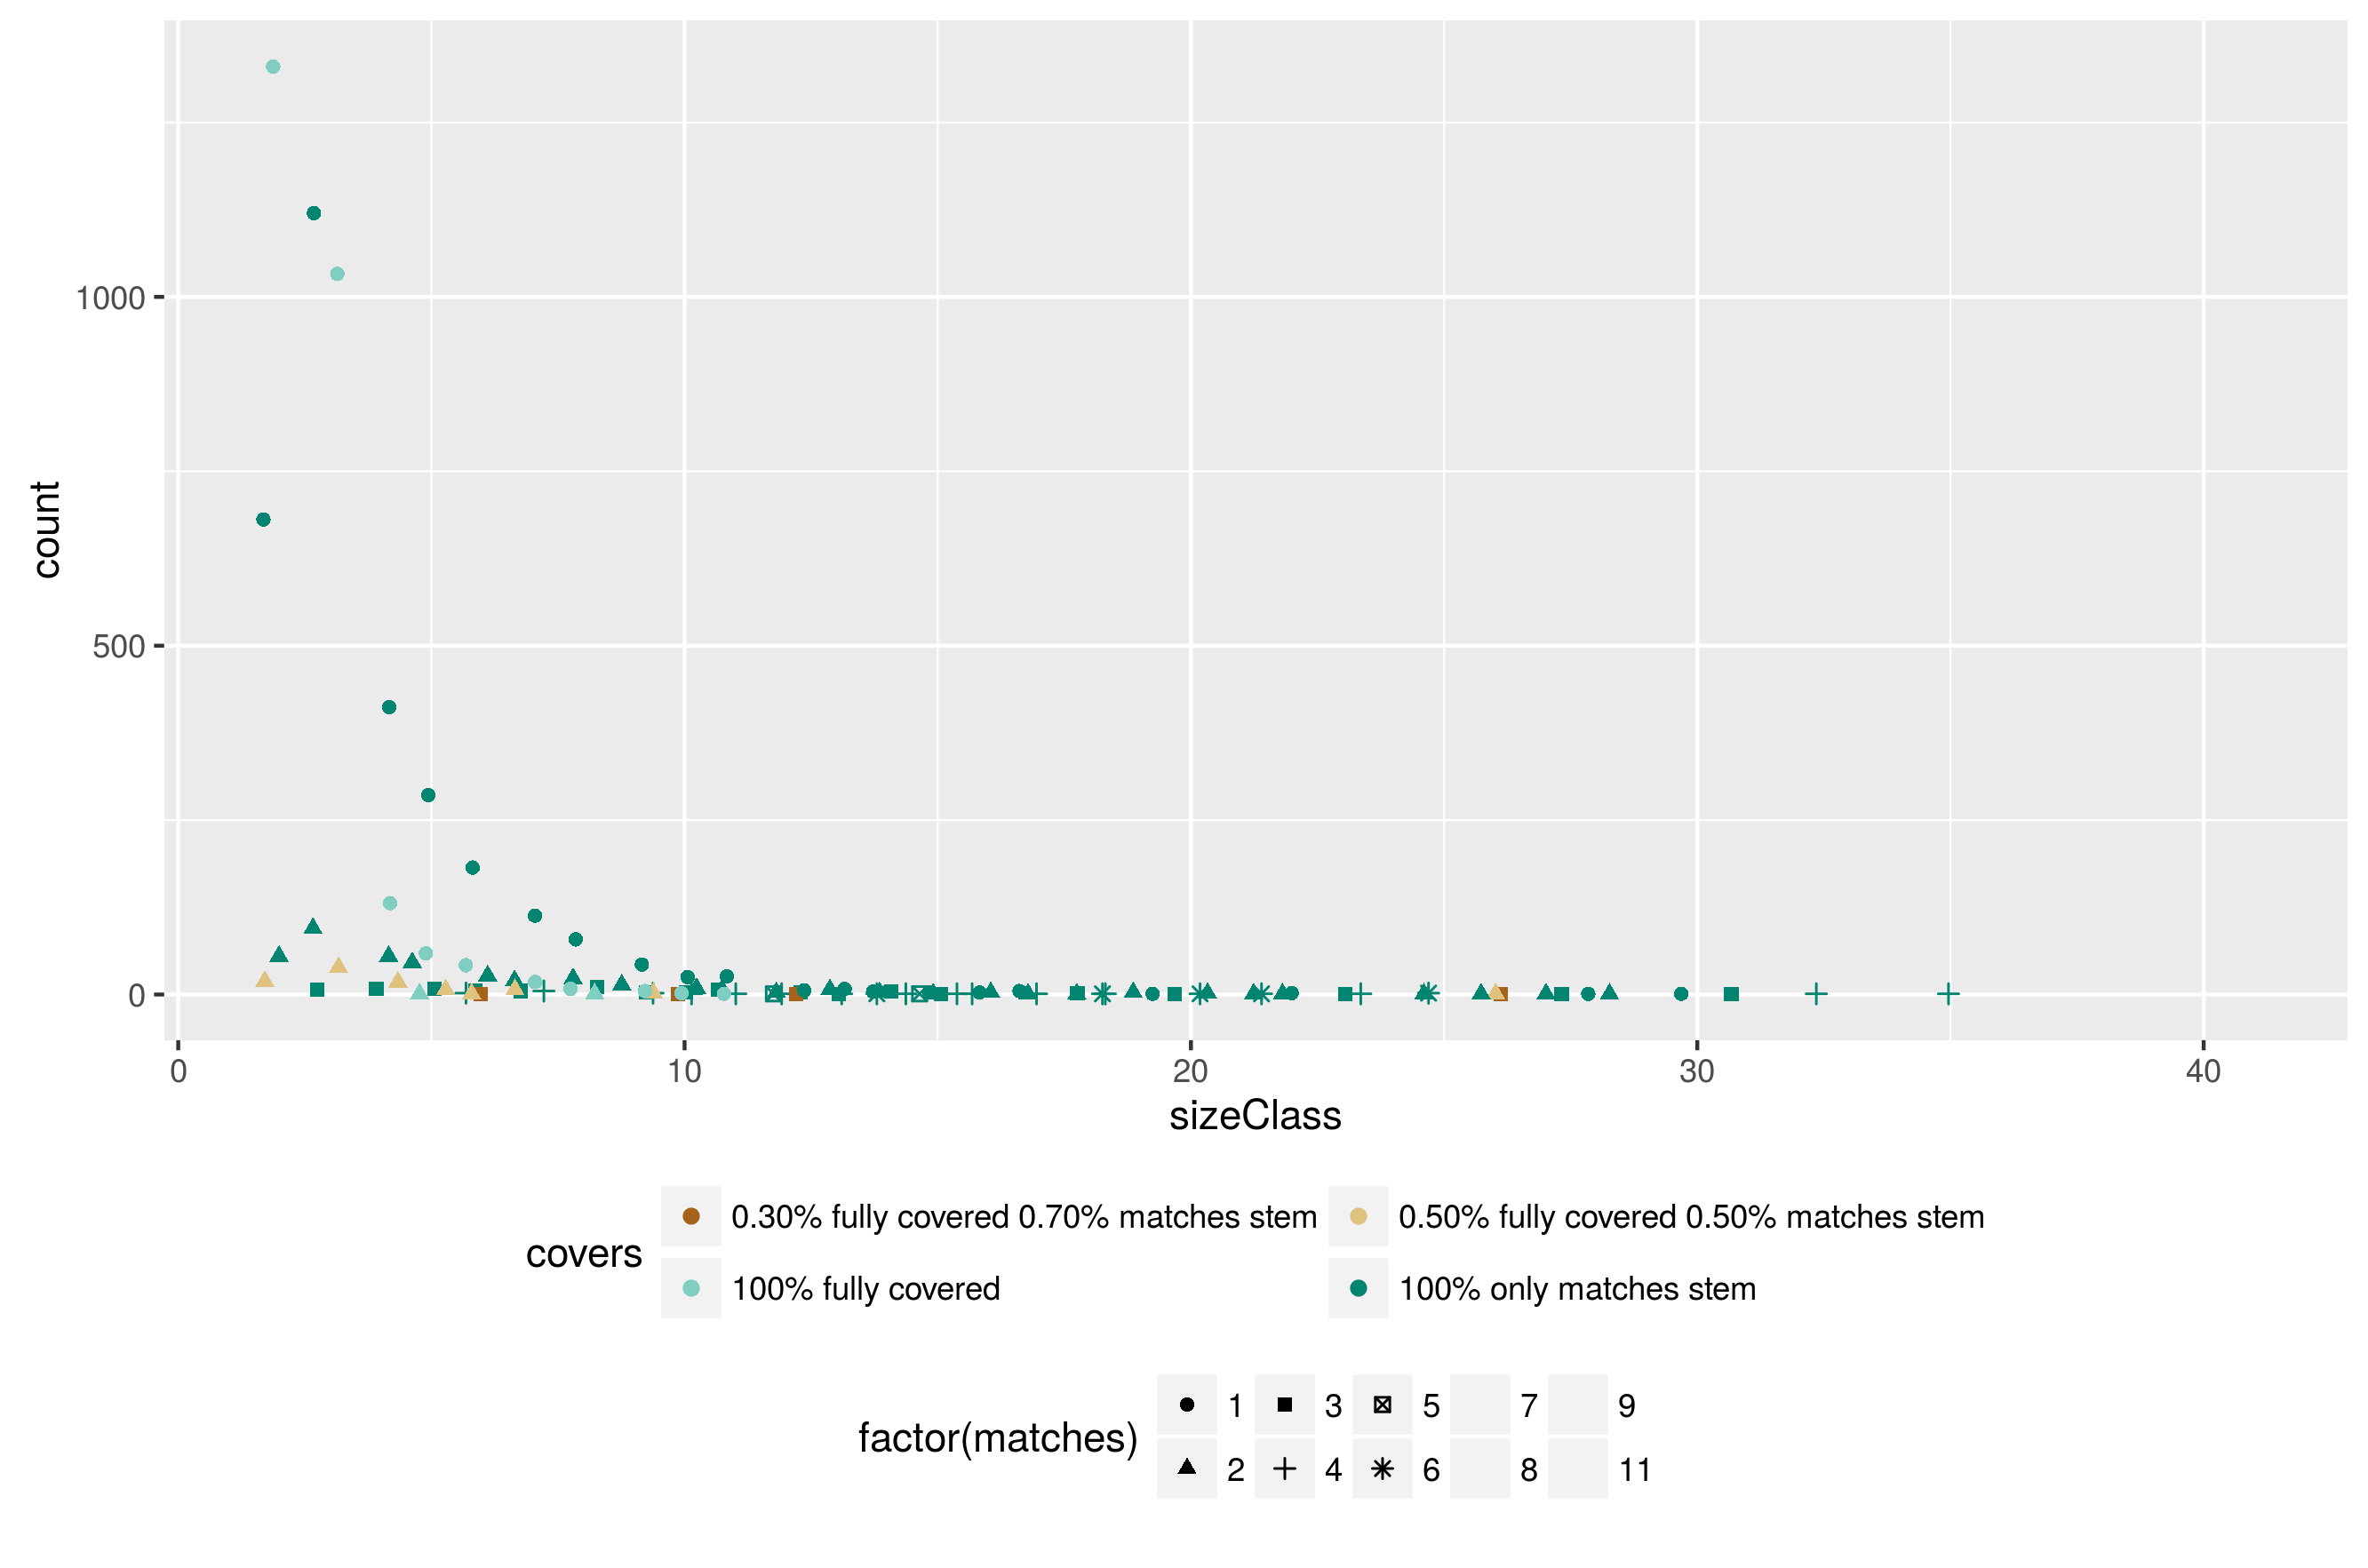
\includegraphics[scale=0.8]{Lancasterconnected.png}
\caption{Lancaster Connected}
\label{fig:lanc}
\end{figure}
\begin{code}
\captionof{listing}{Stem Class From Graph Using Ordered Window} \label{code:gsc}
	\pycode{code/graphStemClass.py}
\end{code}
\newpage
\begin{code}
\captionof{listing}{Run Galago} \label{code:rg}
	\shellcode{code/rungalago.sh}
\end{code}

\newpage
\end{document}